% Selected actual model relationships. QualityAlert has no move_line_id.
\begingroup\setstretch{1}
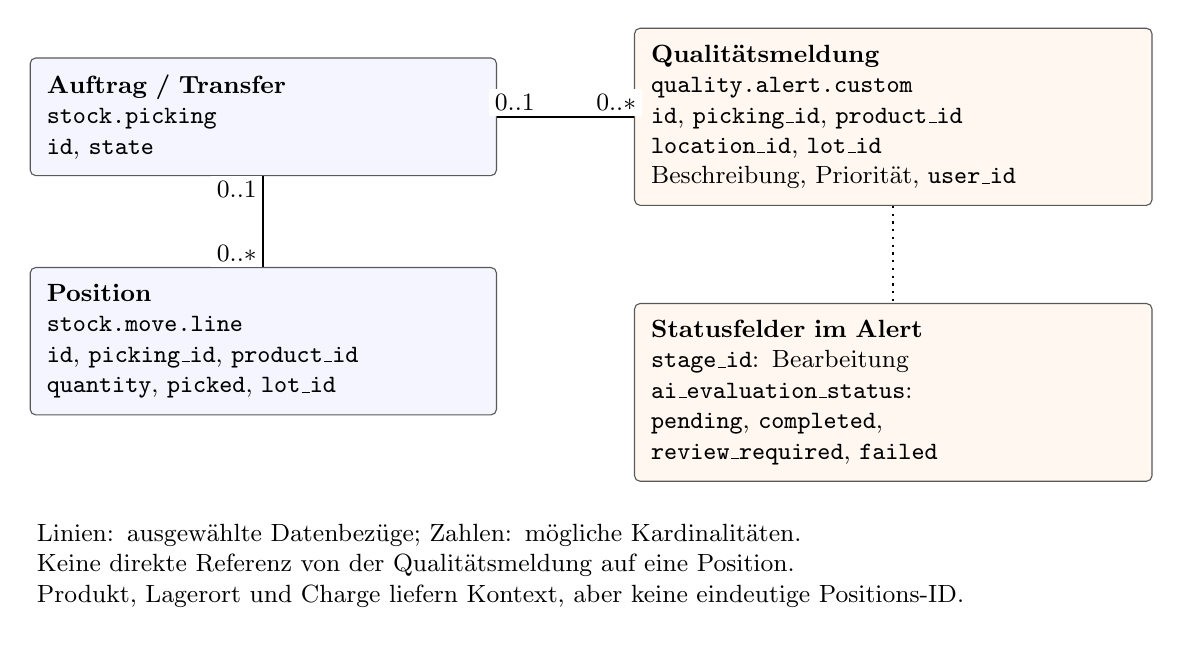
\begin{tikzpicture}[
  font=\small,
  entity/.style={draw=black!65,rounded corners=2pt,align=left,
    text width=5.5cm,inner sep=6pt,fill=blue!4},
  relation/.style={thick},
  lab/.style={font=\small,fill=white,inner sep=2pt}
]
\node[entity] (pick) at (3,0) {\textbf{Auftrag / Transfer}\\
  \texttt{stock.picking}\\
  \texttt{id}, \texttt{state}};
\node[entity] (line) at (3,-2.85) {\textbf{Position}\\
  \texttt{stock.move.line}\\
  \texttt{id}, \texttt{picking\_id}, \texttt{product\_id}\\
  \texttt{quantity}, \texttt{picked}, \texttt{lot\_id}};
\node[entity,text width=6.15cm,fill=orange!6] (alert) at (11,0) {\textbf{Qualitätsmeldung}\\
  \texttt{quality.alert.custom}\\
  \texttt{id}, \texttt{picking\_id}, \texttt{product\_id}\\
  \texttt{location\_id}, \texttt{lot\_id}\\
  Beschreibung, Priorität, \texttt{user\_id}};
\node[entity,text width=6.15cm,fill=orange!6] (state) at (11,-3.5) {\textbf{Statusfelder im Alert}\\
  \texttt{stage\_id}: Bearbeitung\\
  \texttt{ai\_evaluation\_status}:\\
  \texttt{pending}, \texttt{completed},\\
  \texttt{review\_required}, \texttt{failed}};
\draw[relation] (pick.south) -- node[lab,left,pos=.15] {$0..1$}
  node[lab,left,pos=.85] {$0..*$} (line.north);
\draw[relation] (pick.east) -- node[lab,above,pos=.13] {$0..1$}
  node[lab,above,pos=.87] {$0..*$} (alert.west);
\draw[relation,dotted] (alert.south) -- (state.north);
\node[align=left,anchor=north west,text width=14.3cm] at (0,-5.05)
  {Linien: ausgewählte Datenbezüge; Zahlen: mögliche Kardinalitäten.\\
   Keine direkte Referenz von der Qualitätsmeldung auf eine Position.\\
   Produkt, Lagerort und Charge liefern Kontext, aber keine eindeutige Positions-ID.};
\end{tikzpicture}
\endgroup
